% Two-panel model schematic: where the TI field enters the Jansen--Rit column (a) and the
% NMM2 PING circuit with its QIF network (b). Klaus, 2026-10-06. Build:
%   cd figures_src && pdflatex fig_models_ti.tex && cp fig_models_ti.pdf ../figures/
\documentclass[border=3pt]{standalone}
\usepackage[T1]{fontenc}
\usepackage{lmodern,amsmath,amssymb}
\usepackage{tikz}
\usetikzlibrary{arrows.meta,positioning,calc,fit,backgrounds}
\definecolor{neblue}{HTML}{0A4F8C}
\definecolor{nemid}{HTML}{4489C8}
\definecolor{nelight}{HTML}{A8CDE9}
\definecolor{nered}{HTML}{B3361F}
\definecolor{negray}{HTML}{555555}
\definecolor{negreen}{HTML}{1A9850}
\tikzset{
  pop/.style={draw=neblue, line width=0.9pt, rounded corners=3pt, fill=nemid, text=white,
              align=center, minimum width=22mm, minimum height=10mm, font=\small},
  aux/.style={draw=neblue, line width=0.7pt, rounded corners=2pt, fill=nelight, text=neblue,
              align=center, minimum width=21mm, minimum height=9mm, font=\footnotesize},
  exc/.style={-{Stealth[length=2.4mm]}, line width=0.9pt, neblue, rounded corners=3pt},
  inh/.style={-{Circle[length=2mm, open]}, line width=0.9pt, nered, rounded corners=3pt},
  fld/.style={-{Stealth[length=2.4mm]}, line width=1.1pt, negreen},
  lab/.style={font=\footnotesize, text=negray, align=center},
  stage/.style={font=\footnotesize\bfseries, text=nered, align=center},
  title/.style={font=\bfseries, text=neblue, anchor=west},
}
\newcommand{\beaticon}[3]{% x0, y0, width
  \draw[negreen, line width=0.6pt, domain=0:#3, samples=500, smooth, variable=\t]
    plot ({#1+\t}, {#2+0.17*(cos(\t*2400) + cos(\t*2600))});}
\begin{document}
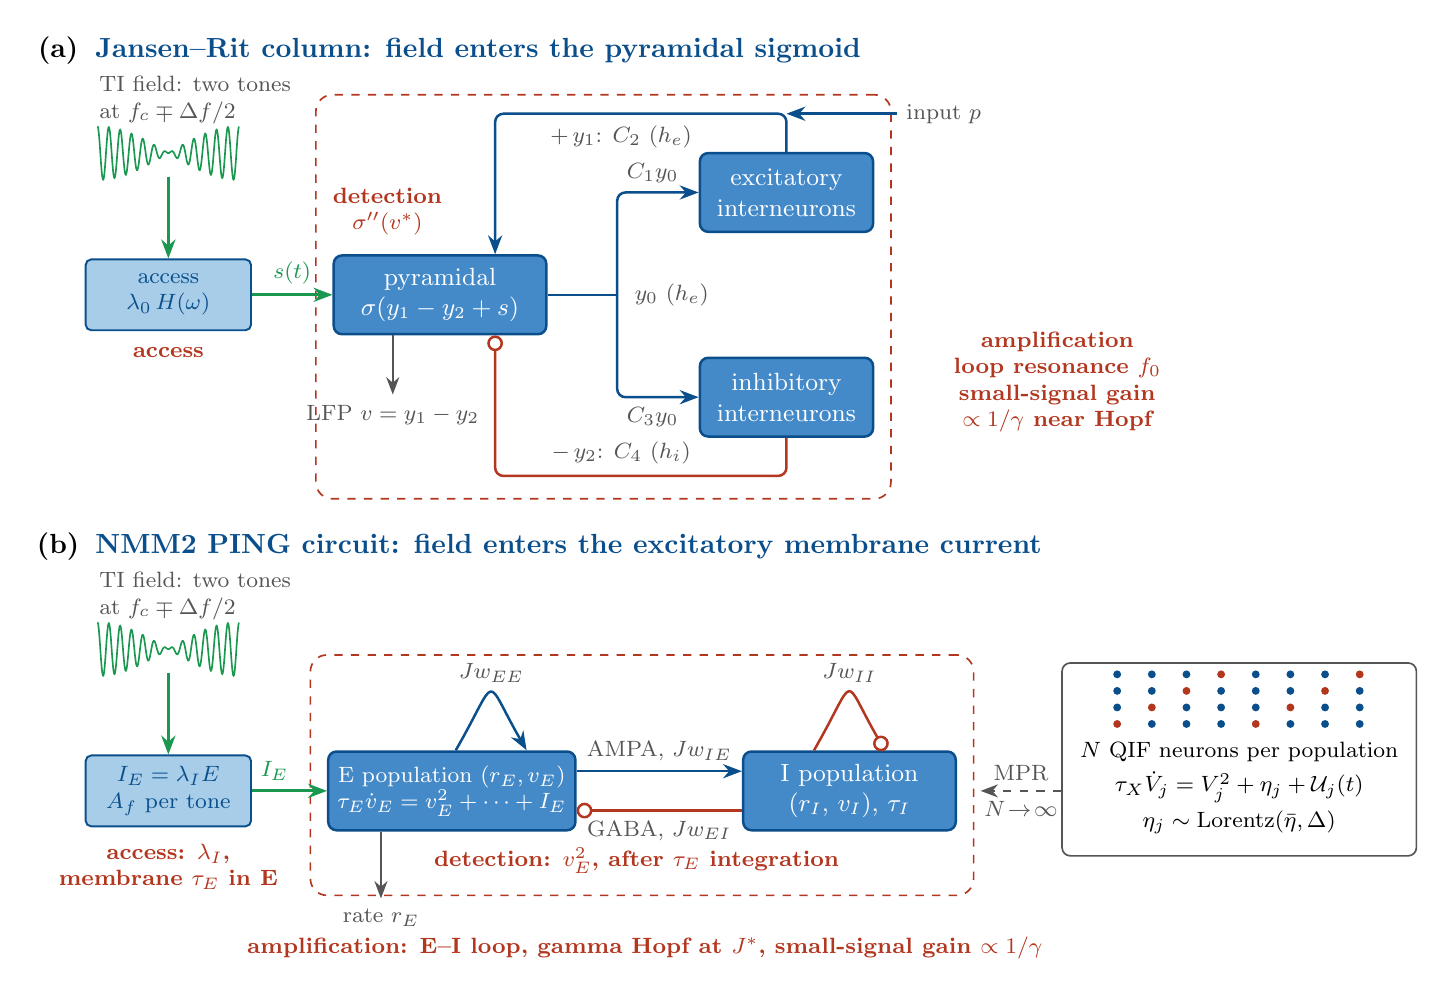
\begin{tikzpicture}[x=1cm, y=1cm]

% ================================================================ (a) Jansen--Rit
\node[font=\bfseries] at (-0.25, 5.45) {(a)};
\node[title] at (0.1, 5.45) {Jansen--Rit column: field enters the pyramidal sigmoid};

\beaticon{0.25}{4.15}{1.8}
\node[lab, anchor=south west, align=left] at (0.15, 4.4) {TI field: two tones\\at $f_c\mp\Delta f/2$};
\node[aux] (accA) at (1.15, 2.35) {access\\$\lambda_0\,H(\omega)$};
\draw[fld] (1.15, 3.85) -- (accA.north);
\node[stage, anchor=north] at (1.15, 1.8) {access};

\node[pop, minimum width=27mm] (P) at (4.6, 2.35) {pyramidal\\$\sigma(y_1-y_2+s)$};
\draw[fld] (accA.east) -- node[above, font=\footnotesize, text=negreen] {$s(t)$} (P.west);
\node[stage, anchor=south east] at ($(P.north)+(0.15,0.12)$) {detection\\$\sigma''(v^*)$};

\node[pop] (EIN) at (9.0, 3.65) {excitatory\\interneurons};
\node[pop] (IIN) at (9.0, 1.05) {inhibitory\\interneurons};

% forward: P -> both interneuron populations (y0 through h_e)
\coordinate (bus) at (6.85, 2.35);
\draw[line width=0.9pt, neblue] (P.east) -- (bus);
\draw[exc] (bus) |- (EIN.west);
\draw[exc] (bus) |- (IIN.west);
\node[lab, anchor=west] at (6.95, 2.35) {$y_0$ ($h_e$)};
\node[lab, anchor=south] at (7.3, 3.65) {$C_1y_0$};
\node[lab, anchor=north] at (7.3, 1.05) {$C_3y_0$};

% feedback
\draw[exc] (EIN.north) |- (5.3, 4.65) -- ($(P.north)+(0.7,0)$);
\node[lab, anchor=north] at (6.9, 4.62) {$+\,y_1$: $C_2$ ($h_e$)};
\draw[inh] (IIN.south) |- (5.3, 0.05) -- ($(P.south)+(0.7,0)$);
\node[lab, anchor=south] at (6.9, 0.08) {$-\,y_2$: $C_4$ ($h_i$)};
\node[lab, anchor=west] (pin) at (10.4, 4.65) {input $p$};
\draw[exc] (pin.west) -- (9.0, 4.65);

% output
\draw[-{Stealth[length=2.2mm]}, line width=0.9pt, negray] ($(P.south)+(-0.6,0)$) -- ++(0,-0.75)
   node[below, lab] {LFP $v=y_1-y_2$};

\coordinate (topA) at (5.3,4.75); \coordinate (botA) at (5.3,-0.1);
\begin{scope}[on background layer]
  \node[draw=nered, dashed, line width=0.6pt, rounded corners=6pt, inner xsep=6pt, inner ysep=4pt,
        fit=(P)(EIN)(IIN)(topA)(botA)] {};
\end{scope}
\node[stage, anchor=north west] at (11.0, 2.0) {amplification\\loop resonance $f_0$\\small-signal gain\\$\propto1/\gamma$ near Hopf};

% ================================================================ (b) NMM2 PING + QIF
\begin{scope}[yshift=-6.3cm]
\node[font=\bfseries] at (-0.25, 5.45) {(b)};
\node[title] at (0.1, 5.45) {NMM2 PING circuit: field enters the excitatory membrane current};

\beaticon{0.25}{4.15}{1.8}
\node[lab, anchor=south west, align=left] at (0.15, 4.4) {TI field: two tones\\at $f_c\mp\Delta f/2$};
\node[aux] (accB) at (1.15, 2.35) {$I_E=\lambda_I E$\\$A_f$ per tone};
\draw[fld] (1.15, 3.85) -- (accB.north);
\node[stage, anchor=north] at (1.15, 1.8) {access: $\lambda_I$,\\membrane $\tau_E$ in E};

\node[pop, minimum width=30mm, font=\footnotesize] (E) at (4.75, 2.35) {E population $(r_E,v_E)$\\$\tau_E\dot v_E=v_E^2+\cdots+I_E$};
\node[pop, minimum width=27mm] (I) at (9.8, 2.35) {I population\\$(r_I,\,v_I)$, $\tau_I$};
\draw[fld] (accB.east) -- node[above, pos=0.3, font=\footnotesize, text=negreen] {$I_E$} (E.west);
\node[stage, anchor=north west] at ($(E.south)+(-0.35,-0.08)$) {detection: $v_E^2$, after $\tau_E$ integration};

\draw[exc] ($(E.east)+(0,0.25)$) -- node[above, lab] {AMPA, $J w_{IE}$} ($(I.west)+(0,0.25)$);
\draw[inh] ($(I.west)+(0,-0.25)$) -- node[below, lab] {GABA, $J w_{EI}$} ($(E.east)+(0,-0.25)$);
\draw[exc] ($(E.north)+(0.05,0)$) to[out=60, in=120, looseness=3.2] node[above, lab] {$J w_{EE}$} ($(E.north)+(0.95,0)$);
\draw[inh] ($(I.north)+(-0.45,0)$) to[out=60, in=120, looseness=3.2] node[above, lab] {$J w_{II}$} ($(I.north)+(0.45,0)$);

\draw[-{Stealth[length=2.2mm]}, line width=0.9pt, negray] ($(E.south)+(-0.9,0)$) -- ++(0,-0.85)
   node[below, lab] {rate $r_E$};

\coordinate (topB) at ($(E.north)+(0,1.0)$); \coordinate (botB) at ($(I.south)+(0,-0.6)$);
\begin{scope}[on background layer]
  \node[draw=nered, dashed, line width=0.6pt, rounded corners=6pt, inner xsep=6pt, inner ysep=6pt,
        fit=(E)(I)(topB)(botB)] (loopB) {};
\end{scope}
\node[stage, anchor=north] at (7.2, 0.62) {amplification: E--I loop, gamma Hopf at $J^*$, small-signal gain $\propto1/\gamma$};

% QIF inset
\node[draw=negray, line width=0.6pt, rounded corners=3pt, fill=white, minimum width=4.5cm,
      minimum height=2.45cm] (qbox) at (14.75, 2.75) {};
\foreach \i in {0,...,7}{\foreach \j in {0,...,3}{
  \pgfmathtruncatemacro{\c}{mod(\i+3*\j,4)==0 ? 1 : 0}
  \ifnum\c=1 \fill[nered] (13.2+0.44*\i, 3.2+0.21*\j) circle (0.05);
  \else \fill[neblue] (13.2+0.44*\i, 3.2+0.21*\j) circle (0.05); \fi }}
\node[lab, text=black] at (14.75, 2.85) {$N$ QIF neurons per population};
\node[lab, text=black] at (14.75, 2.4) {$\tau_X\dot V_j=V_j^2+\eta_j+\mathcal U_j(t)$};
\node[lab, text=black] at (14.75, 1.95) {$\eta_j\sim\mathrm{Lorentz}(\bar\eta,\Delta)$};
\draw[-{Stealth[length=2.2mm]}, line width=0.8pt, negray, dashed] (qbox.west |- I.east) --
   node[above, lab] {MPR} node[below, lab] {$N\!\to\!\infty$} ($(I.east)+(0.3,0)$);
\end{scope}
\end{tikzpicture}
\end{document}
